\section{Lab: Page tables}
\subsection{实验目的}

本实验中将涉及到操作系统中重要的\textbf{页表}概念。操作系统中的页表是一种数据结构,用于实现虚拟内存和物理内存之间的地址映射。每个进程都有自己的页表,将虚拟地址映射到物理地址,从而使得操作系统能够有效地管理内存,提供内存保护和共享内存功能。页表的概念对于操作系统课程至关重要,因为它涉及到内存管理、进程隔离和系统性能等核心问题。理解页表如何工作,有助于深入掌握操作系统的内存管理机制,了解虚拟内存的实现细节,并且能够解决与内存管理相关的各种问题。

本实验中将探索页表的具体操作并对其进行修改,以加快某些系统调用并检测哪些页面被访问。具体将实现以下内容:
\begin{itemize}
    \item 利用页表加速系统调用;
    \item 打印页表;
    \item 检测被访问的页表。
\end{itemize}

\subsection{实验步骤}

\subsubsection{实现系统调用加速}
\begin{enumerate}
    \item 首先,在proc.c文件中修改proc\_pagetable函数,仿照前面的代码添加用户页表的映射,注意内存权限应为PTE\_U。
          \begin{lstlisting}[language=c, title=对proc\_pagetable函数的修改]
    pagetable_t proc_pagetable(struct proc *p)
    {
        pagetable_t pagetable;

        ...

        // 添加的部分
        if (mappages(pagetable, USYSCALL, PGSIZE,
                    (uint64)(p->usyscall), PTE_R | PTE_U) < 0)
        {
            uvmunmap(pagetable, USYSCALL, 1, 0);
            uvmunmap(pagetable, TRAMPOLINE, 1, 0);
            uvmfree(pagetable, 0);
            return 0;
        }

        return pagetable;
    }
    \end{lstlisting}
    \item 在proc.c文件中修改allocproc函数,仿照前面的代码,给进程分配用户页表。
          \begin{lstlisting}[language=c, title=对allocproc函数的修改]
    static struct proc * allocproc(void)
    {
        ...
    
        // 添加的部分
        if ((p->usyscall = (struct usyscall *)kalloc()) == 0)
        {
            freeproc(p);
            release(&p->lock);
            return 0;
        }
        p->usyscall->pid = p->pid;
    
        ...

        return p;
    }
    \end{lstlisting}
    \item 在proc.c文件中修改freeproc函数,仿照前面的代码,释放用户页表。
          \begin{lstlisting}[language=c, title=对freeproc函数的修改]
    freeproc(struct proc *p)
    {
        ...
        // 添加的部分
        if (p->usyscall)
        kfree((void *)p->usyscall);
        p->usyscall = 0;
        ...
    }
    \end{lstlisting}
    \item 如此设置,系统就能利用用户页表实现更快地进程号查询,从而加速系统调用。
\end{enumerate}

\subsubsection{实现页表打印}
\begin{enumerate}
    \item 首先,阅读vm.c文件中freewalk函数的代码,了解如何对页表项进行递归遍历和访问。
          \begin{lstlisting}[language=c, title=freewalk函数的原型]
    // Recursively free page-table pages.
    // All leaf mappings must already have been removed.
    void freewalk(pagetable_t pagetable)
    {
        // there are 2^9 = 512 PTEs in a page table.
        for (int i = 0; i < 512; i++)
        {
            pte_t pte = pagetable[i];
            if ((pte & PTE_V) && (pte & (PTE_R | PTE_W | PTE_X)) == 0)
            {
                // this PTE points to a lower-level page table.
                uint64 child = PTE2PA(pte);
                freewalk((pagetable_t)child);
                pagetable[i] = 0;
            }
            else if (pte & PTE_V)
            {
                panic("freewalk: leaf");
            }
        }
        kfree((void *)pagetable);
    }
    \end{lstlisting}
    \item 仿照freewalk函数,实现递归打印页表的vmprint函数
          \begin{lstlisting}[language=c, title=vmprint函数的实现]
    void vmprint(pagetable_t pagetable, uint64 depth)
    {
        // 如果递归深度大于2,则直接返回,RISC-V只有三级页表
        if (depth > 2)
        return;
    
        // 如果是最顶层页表,打印页表的地址
        if (depth == 0)
        {
            printf("page table %p\n", pagetable);
        }
    
        // 定义一个静态的前缀数组,用于打印格式化输出
        static char *prefix[] = {"..", ".. ..", ".. .. .."};
    
        // 页表中有2^9 = 512个页表项
        for (int i = 0; i < 512; i++)
        {
            pte_t pte = pagetable[i];  // 获取当前页表项
            if (pte & PTE_V)  // 如果页表项有效
            {
                // 打印当前页表项的信息,包括前缀、索引、页表项和物理地址
                printf("%s%d: pte %p pa %p\n", prefix[depth], i, pte, PTE2PA(pte));
                uint64 child = PTE2PA(pte);  // 获取下一级页表的物理地址
                vmprint((pagetable_t)child, depth + 1);  // 递归打印下一级页表
            }
        }
    }
    \end{lstlisting}
    \item 在def.h中声明vmprint函数以便调用。
    \item 在exec.c文件中,对exec函数进行修改,调用vmprint函数,使其在进程号为1是打印页表。
          \begin{lstlisting}[language=c, title=对exec函数的修改]
    int exec(char *path, char **argv)
    {
        ...
        
        // 添加的语句
        if (p->pid == 1)
            vmprint(p->pagetable, 0);

        ...
    }    
    \end{lstlisting}
\end{enumerate}
\subsubsection{实现被访问页面侦测}
\begin{enumerate}
    \item 首先,在riscv.h文件中添加一个PTE\_A常量,查阅RISC-V手册可知其值应为0b00100000,即$2^6$。
          \begin{lstlisting}[language=c, title=PTE\_A的定义]
    #define PTE_A (1L << 6)    
    \end{lstlisting}
    \item 在vm.c文件中实现vm\_pgaccess函数,利用PTE\_A标志判断给定虚拟地址的页表项是否被访问,若被访问返回1并清除PTE\_A标志。在def.h中添加函数的声明。
          \begin{lstlisting}[language=c, title=vm\_pgaccess函数的实现]
    int vm_pgaccess(pagetable_t pagetable, uint64 va)
    {
        pte_t *pte;  // 页表项指针
    
        // 如果虚拟地址超出最大允许值,返回0
        if (va >= MAXVA)
            return 0;
    
        // 获取虚拟地址对应的页表项指针
        pte = walk(pagetable, va, 0);
        // 如果页表项不存在,返回0
        if (pte == 0)
            return 0;
    
        // 如果页表项的访问标志位被设置
        if ((*pte & PTE_A) != 0)
        {
            // 清除访问标志位
            *pte = *pte & (~PTE_A);
            // 返回1表示访问标志位被清除
            return 1;
        }
    
        // 如果访问标志位未设置,返回0
        return 0;
    }
    \end{lstlisting}
    \item 在sysproc.c中补全sys\_pgaccess系统调用,使之能够把页面访问的情况记录在掩码之中。
          \begin{lstlisting}[language=c, title=sys\_pgaccess函数的实现]
    int sys_pgaccess(void)
    {
        uint64 addr;  // 内存起始地址
        int len;      // 内存区域的页数
        int bitmask;  // 存储结果的用户地址
    
        // 获取系统调用的第一个参数(内存起始地址),并检查是否成功
        if (argaddr(0, &addr) < 0)
            return -1;
    
        // 获取系统调用的第二个参数(内存区域的页数),并检查是否成功
        if (argint(1, &len) < 0)
            return -1;
    
        // 获取系统调用的第三个参数(存储结果的用户地址),并检查是否成功
        if (argint(2, &bitmask) < 0)
            return -1;
    
        // 检查页数是否在合理范围内(0到32页)
        if (len > 32 || len < 0)
            return -1;
    
        int res = 0;  // 用于存储访问标志结果
        int i;
        struct proc *p = myproc();  // 获取当前进程结构体
    
        // 遍历每一页,检查访问标志并存储结果
        for (i = 0; i < len; i++)
        {
            int va = addr + i * PGSIZE;  // 计算每一页的虚拟地址
            int abit = vm_pgaccess(p->pagetable, va);  // 检查页表项的访问标志
        
            res = res | abit << i;  // 将访问标志结果合并到res中
        }
    
        // 将结果拷贝到用户空间,如果失败则返回-1
        if (copyout(p->pagetable, bitmask, (char *)&res, sizeof(res)) < 0)
            return -1;
    
        // 成功返回0
        return 0;
    }      
    \end{lstlisting}
\end{enumerate}

\subsection{评测结果}
利用 grade-lab-pgtbl 脚本评测,得到评测结果如图\ref{fig:pgtbl}所示。
\begin{figure}[h]
    \centering
    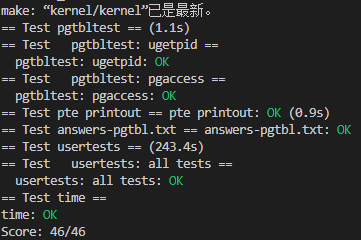
\includegraphics[width=\linewidth]{pics/pagetable评测结果.png}
    \caption{评测结果}
    \label{fig:pgtbl}
\end{figure}

\subsection{实验小结}
在本次实验中,我深入探索了操作系统中的页表概念,并通过一系列具体的实现来加深对该概念的理解。页表是操作系统中管理虚拟内存的重要数据结构,它通过将虚拟地址映射到物理地址,实现内存保护和内存共享功能。我通过本实验的操作,掌握了页表的操作方法和实现细节。

我在本实验上花费了不少时间,复习了操作系统课上讲过的页表概念,并研究内核代码。实验总体来说是有些难度。

在实验过程中,我不仅巩固了操作系统中页表的基本概念,还通过实际编程和调试,掌握了页表的具体实现方法和应用场景。通过这些实践操作,我更深入地理解了操作系统的内存管理机制,并积累了宝贵的编程经验和调试技巧。这些知识和技能对于我后续解决实际问题将大有裨益。
